\documentclass[12pt]{article}
\usepackage{graphicx}
\usepackage{subcaption}
\usepackage{mwe}
\usepackage[]{mcode}
%\usepackage{lingmacros}
%\usepackage{tree-dvips}
%\usepackage{blindtext}
%\usepackage[utf8]{inputenc}

\renewcommand{\thesubsection}{\thesection.\alph{subsection}}

\begin{document}

\title{ENPM661 - Augmented Reality}
\author{Gudjon Einar Magnusson}

\maketitle

\section{Tag detection and decoding}

My tag detection algorithm is largely based on the AprilTag implementation described in \cite{apriltag}. The process is split into 3 steps, line detection, quad detection and tag decoding. I will now describe each of these steps in more detail.

\subsection{Line Detection}

The first step is to find the lines that form the edges of the tag. To to this I first find the gradient direction and magnitude of every pixel and threshold it to only consider edges with a very strong gradient. Next I find connected line segments with similar gradient direction, within a small margin. To get a accurate straight line I fit a straight line through all the pixels that form a line segment. For each line segment I keep track if its start and end point and a normal that is based on the gradient direction. I make sure that the normal always points form light to dark.

Figure \ref{fig_lines} shows an example of lines that have been fit to edges in the image.

\begin{figure}
    \center
    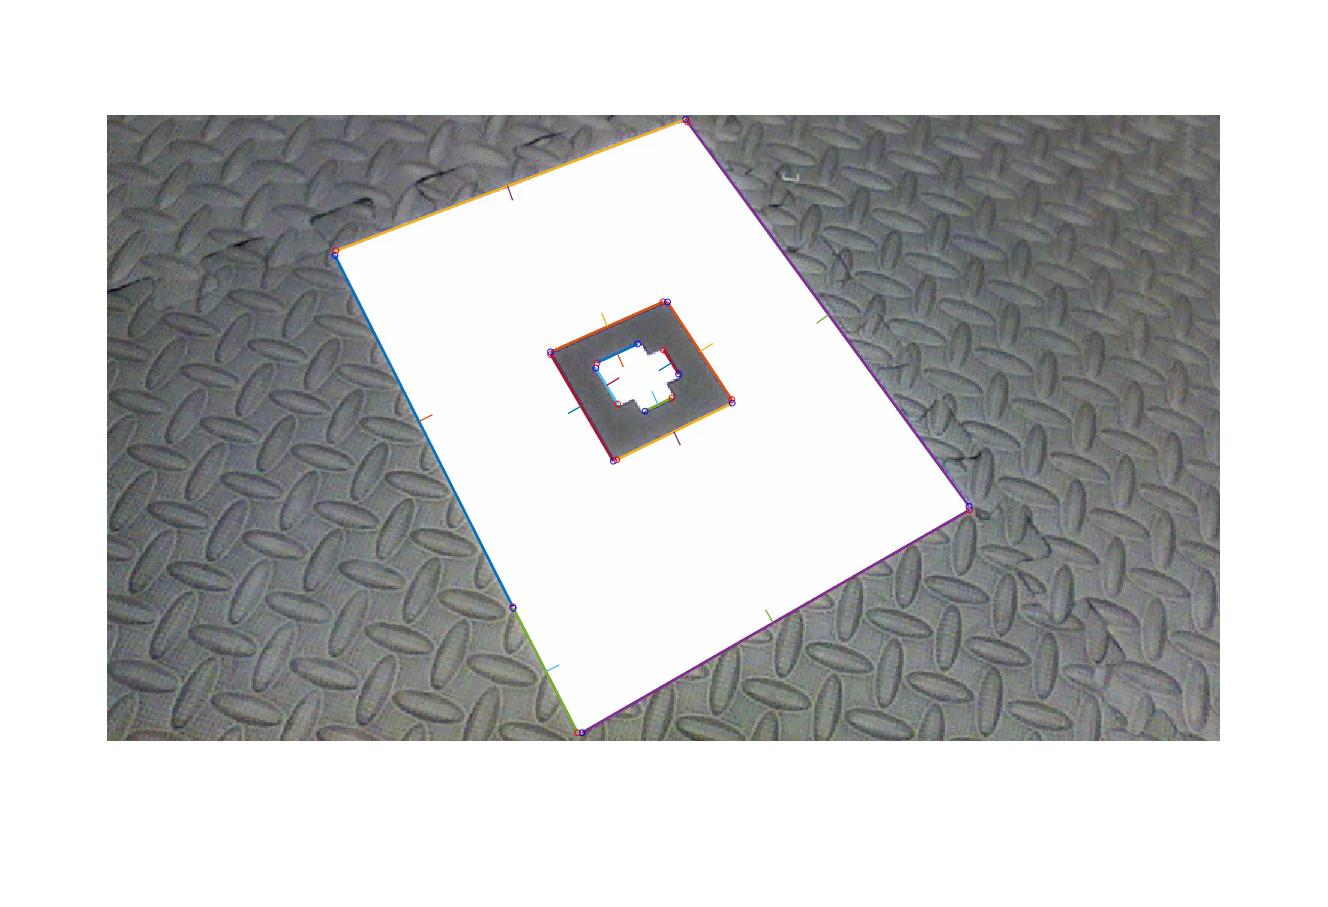
\includegraphics[width=\linewidth]{img/Lines}
    \caption{Line Segments and their normal}
    \label{fig_lines}
\end{figure}


\subsection{Quad Detection}

One lines have been discovered, the next step is to find quads that form a tag. A quad is made out of four lines with normals pointing away from its center. These four lines are found using depth first search that at depth one accepts any line but at later depths, only considers segments that are within a short distance of the previous line end point and the normal is rotated counter clockwise.

The four corners of the tag are the intersection points of the line segments.

\subsection{Tag Decoding}

Once I have found four lines that form a quad I assume its a tag, but I don't know its orientation or id. To decode the tag I use the four corners to find a homography that will project the quad onto a unit square. Next I use that homography to create a small 32 by 32 rectified image of the tag. I find the orientation of the tag by finding which corner has the greatest amount of white pixels, and rotate the tag according to that such that the corner is in the lower right of the image.

I decode the tag by counting the number of white pixels within the sub-squares of the tag and checking if they are above a threshold. If so, its counted as a 1 bit, else its a 0 bit.

Figure \ref{fig_tag} shows a decoded and annotated tag.

\begin{figure}
    \center
    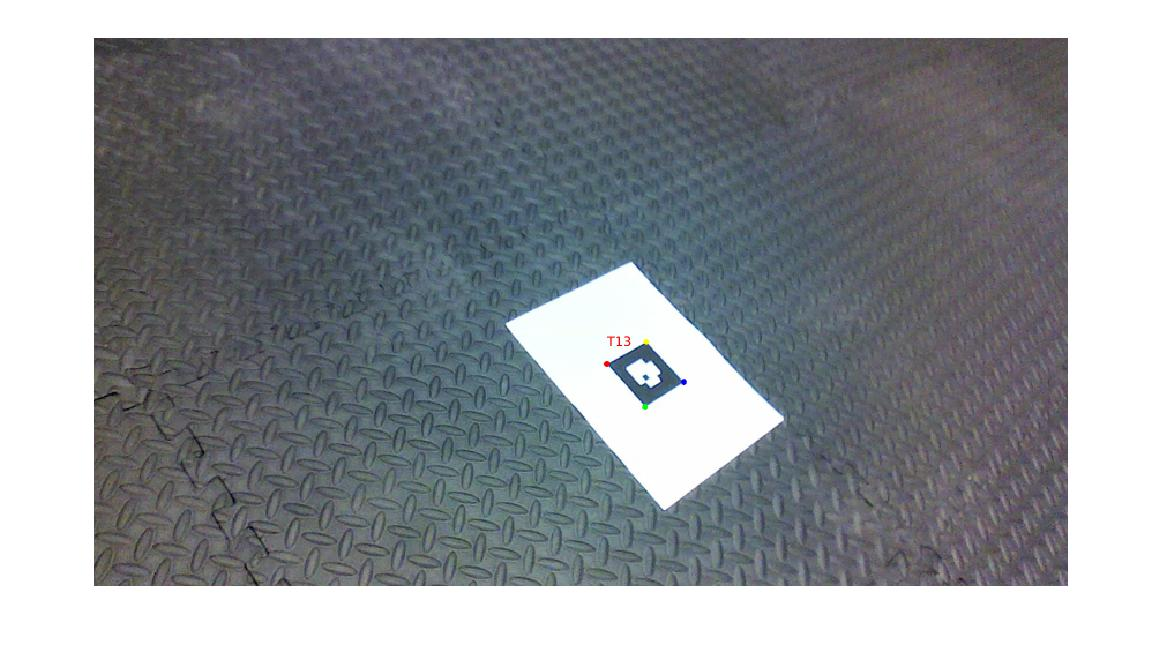
\includegraphics[width=\linewidth]{img/Tag}
    \caption{A tag has been replaced by Lena}
    \label{fig_tag}
\end{figure}


\section{Tag replacement}

Once the tag has be detected and decoded it can easily be replaced by using the inverse of the homography used to rectify the tag.

Figure \ref{fig_lena} shows how Lena has been project on top of a tag.

\begin{figure}
    \center
    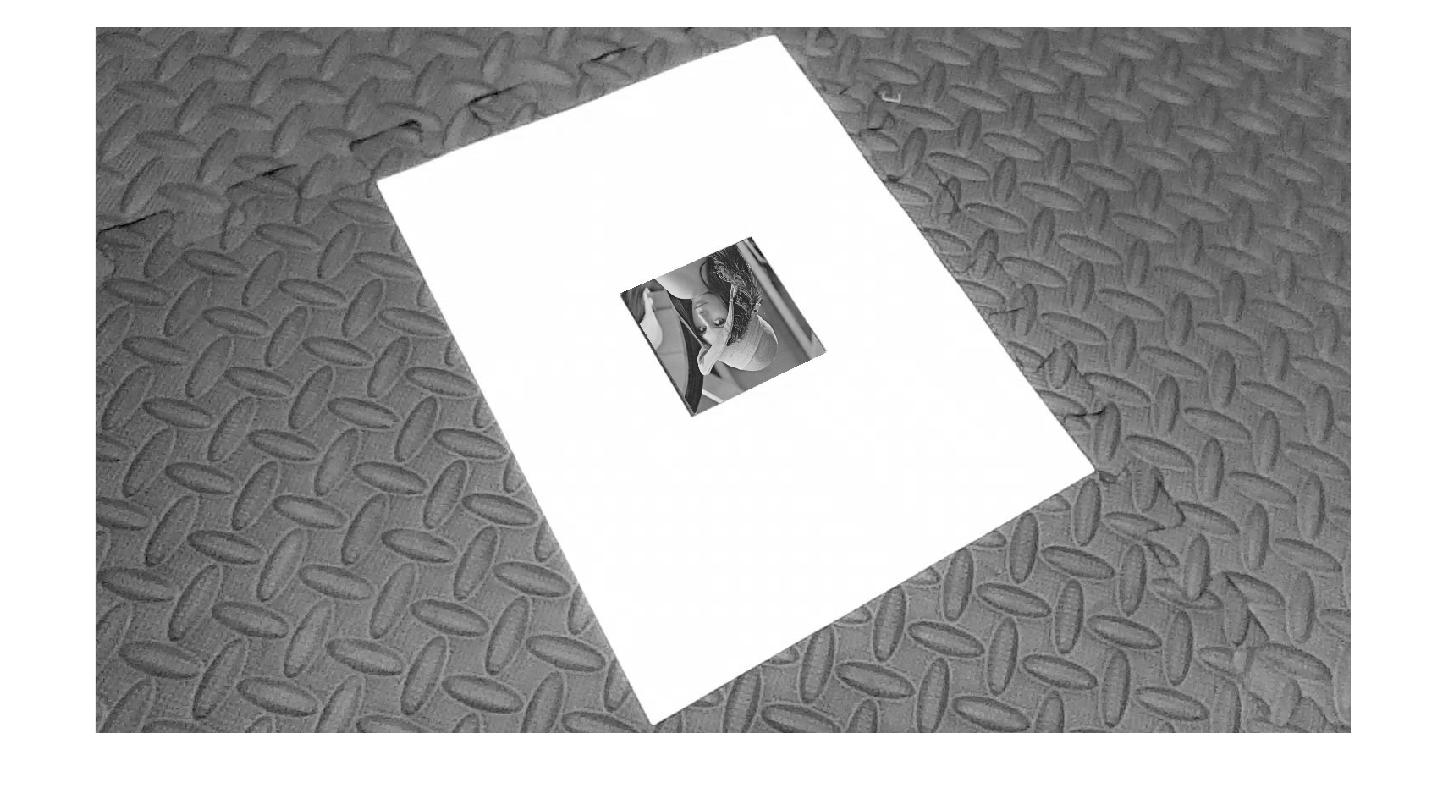
\includegraphics[width=\linewidth]{img/Lena}
    \caption{A tag has been replaced by Lena}
    \label{fig_lena}
\end{figure}


\section{Camera pose from homography}

Using the homography and the intrinsic parameters of the camera we should be able to infer the pose of the camera. That can then be used to draw a cube on top of the cube. 

For a long time I was not able to get this to work. My Z-axis was alway crooked for some reason, as can be seen in figure \ref{fig_proj}. Turn out I had the wrong camera parameters.

Once I got the correct parameters, drawing the cube got a lot easier. The cube can be seen in figure \ref{fig_cube}. 

\begin{figure}
    \center
    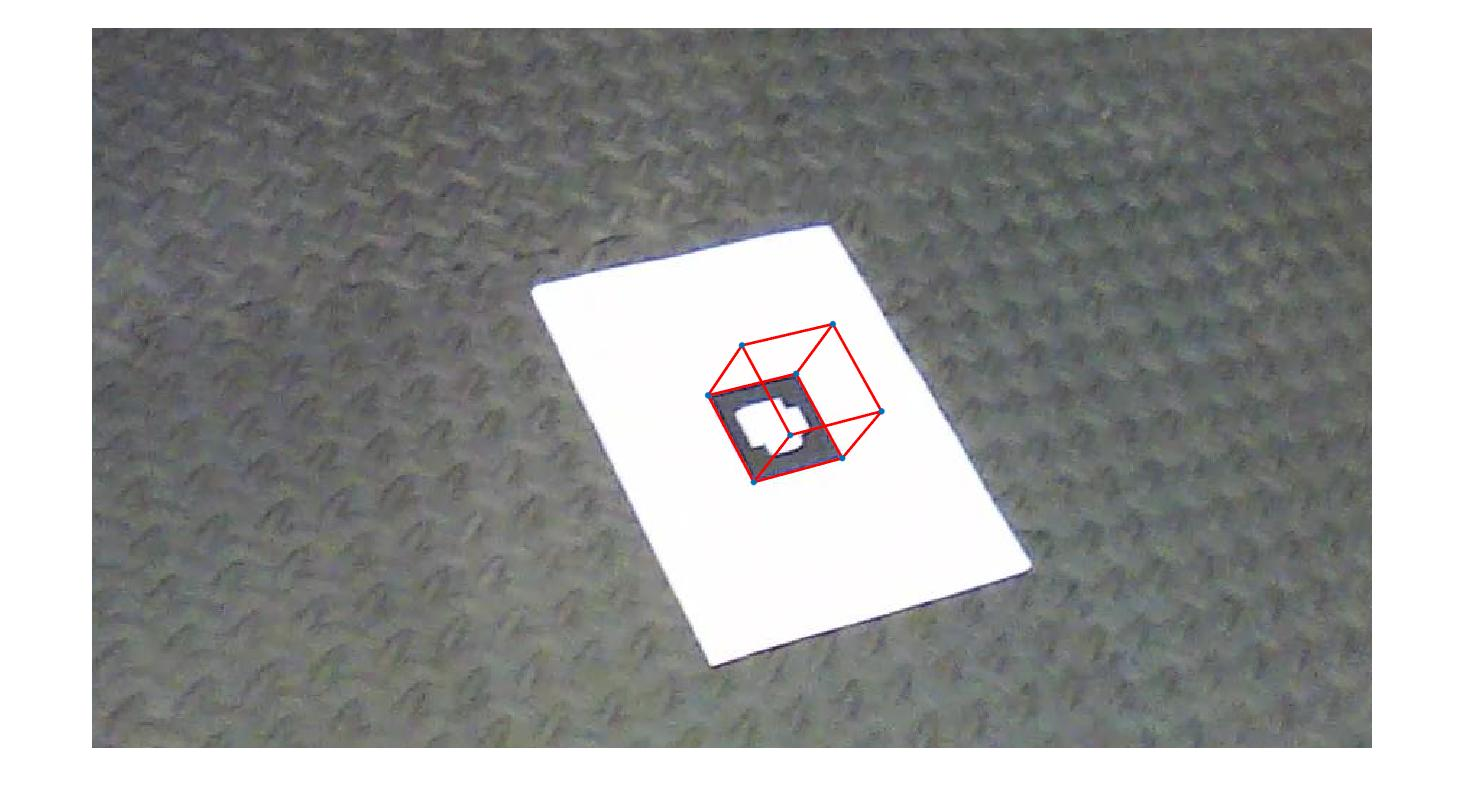
\includegraphics[width=\linewidth]{img/Cube}
    \caption{Given the correct camera parameters, drawing the cube was easy}
    \label{fig_cube}
\end{figure}

\begin{figure}
    \center
    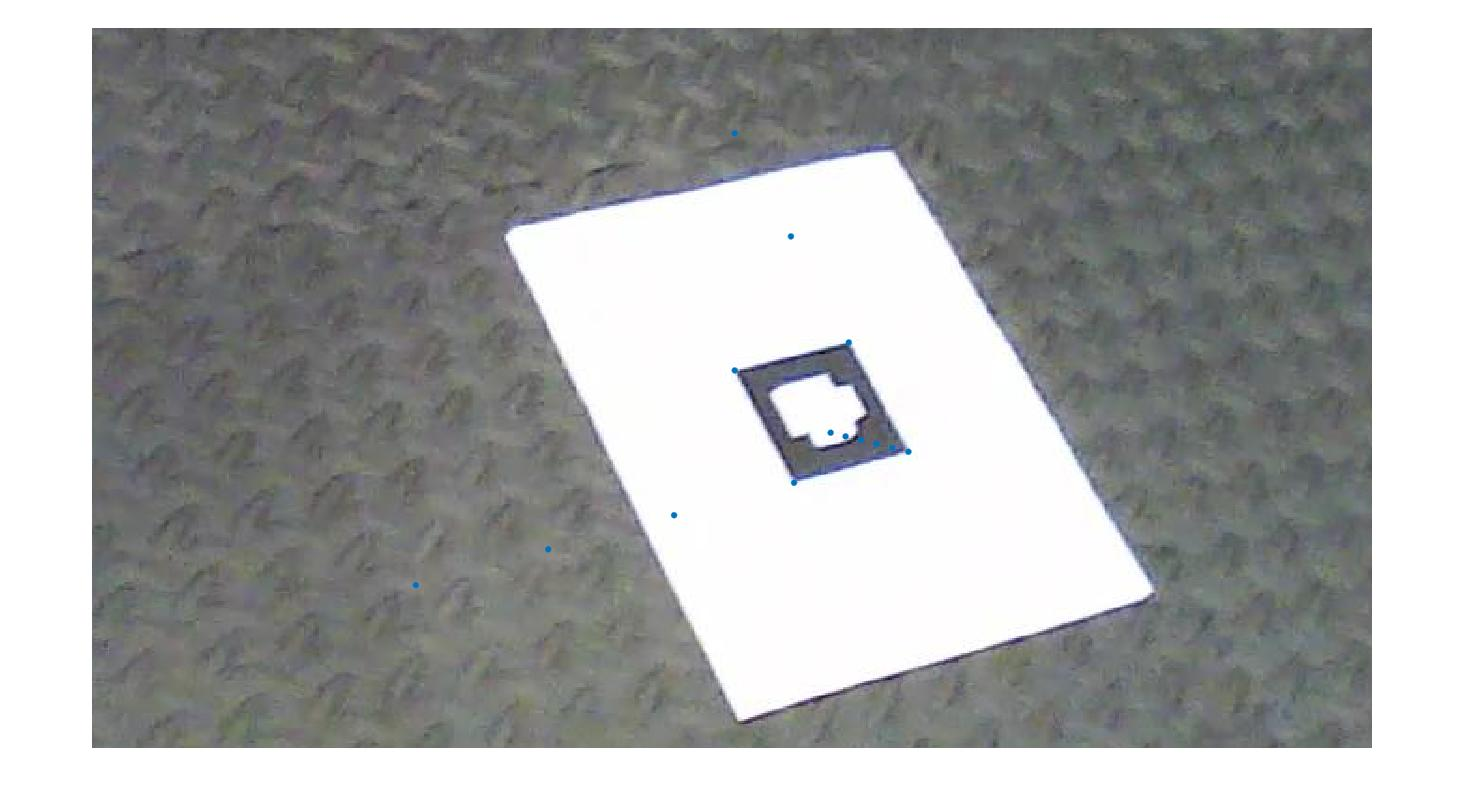
\includegraphics[width=\linewidth]{img/Projection}
    \caption{For some reason my Z-axis is crooked}
    \label{fig_proj}
\end{figure}

\begin{thebibliography}{9}

\bibitem{apriltag}
  Edwin Olson
  \emph{AprilTag: A robust and flexible visual fiducial system}

\end{thebibliography}

\end{document}